\chapter[Related OSS Projects]{Related OSS\\Projects}%
\label{c:rel_projects}%
This chapter looks at other projects from the open source software and open source hardware community which have the goal to develop their own 3D scanners\marginWarning[Important Notice]{It should be noted that the list of projects considered in this chapter does not claim to be exhaustive. In particular, there are various variations for the presented projects and the projects itself may already be a variation of an existing project.}. In some places comparisons to the Open3DScanner are given and influences that the projects have on the Open3DScanner are pointed out.%

In the sections~\ref{s:open_scan} and~\ref{s:3dTurn} other photogrammetry scanners are introduced while in the remaining sections 3D scanners based on other technologies are introduced.%

\section{OpenScan}%
\label{s:open_scan}%
First of all lets take a look at the project that had the biggest influence on the Open3DScanner, because it served as inspiration for it. The Open3DScanner is only an alternative realization of Thomas Megel's project:%

\hrefIdx{https://www.openscan.eu/}{OpenScan}%
\marginElement{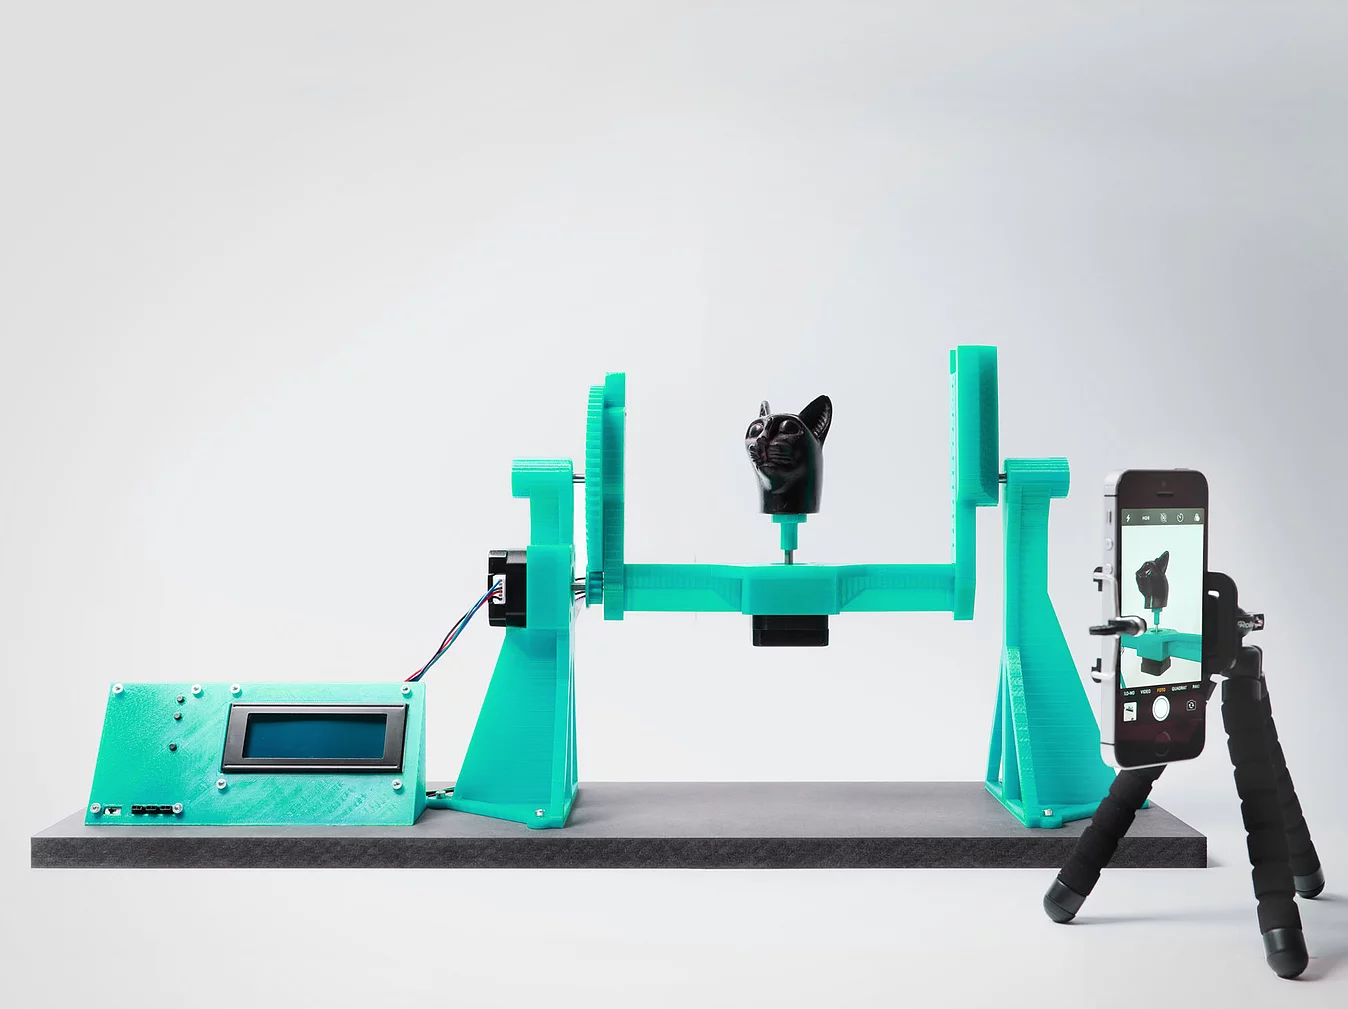
\includegraphics[width=\linewidth]{images/OpenScan.png}\captionof{figure}{The OpenScan 3D Scanner}}%

OpenScan is based on automatically rotating the object to be scanned on two axes (X and Z) while automatically shooting the photos.%

The OpenScan project, like the Open3DScanner, relies on existing cameras that are connected to the scanner. One possibility that OpenScan offers, but was omitted from the Open3DScanner, is the usage of various SLR cameras for 3D scanning. The SLR camera is connected to the scanner via an infrared remote shutter which is connected to the scanner via an optocoupler. This option was removed for the Open3DScanner, because I don't own a SLR camera, nor do I plan to buy one. Furthermore, I am convinced that the quality of modern smartphone cameras is sufficient for the production of good quality 3D scans.%

A feature of the Open3DScanner that OpenScan does not provide is the possibility to connect LED lights directly to the 3D scanner and let the hardware control them during the scanning process.%

While there is no information about the applicable license on the project's homepage, the \hrefIdx{https://www.thingiverse.com/thing:3050437}{OpenScan Thingiverse project} indicates that the project is published under the CC-BY-NC 3.0 license.%

Scans with the OpenScan 3D Scanner are performed fully automatically after the settings for the respective scan have been selected. It is possible to configure how many images are taken per rotation of the z-axis and by which angle the scanner should rotate on the x-axis. In addition, it is possible to determine at how many positions on the x-axis a stop should be made, which in turn results in a complete rotation of the z-axis.%

In addition, there is a setting to adjust the time the scanner stops for each photo. This is important to ensure that the camera can refocus if necessary and avoid blurry shots.%

\infoInfo{Note}{Although the Open3DScanner was developed on the basis of the OpenScan project, it is not a simple copy. After OpenScan motivated the development of the Open3DScanner, requirements were defined independently from the original project. All artifacts (3D models, firmware, BOM) were developed especially for the Open3DScanner.}%

\section{3D Scanner Turntable}%
\label{s:3dTurn}%
Another open source photogrammetry 3D scanner is the project 3D Scanner Turntable by Dave Clarke.%

\hrefIdx{https://www.hackster.io/daveclarke/3d-scanner-turntable-for-cell-phones-updated-64fdb8}{3D Scanner Turntable}%
\marginElement{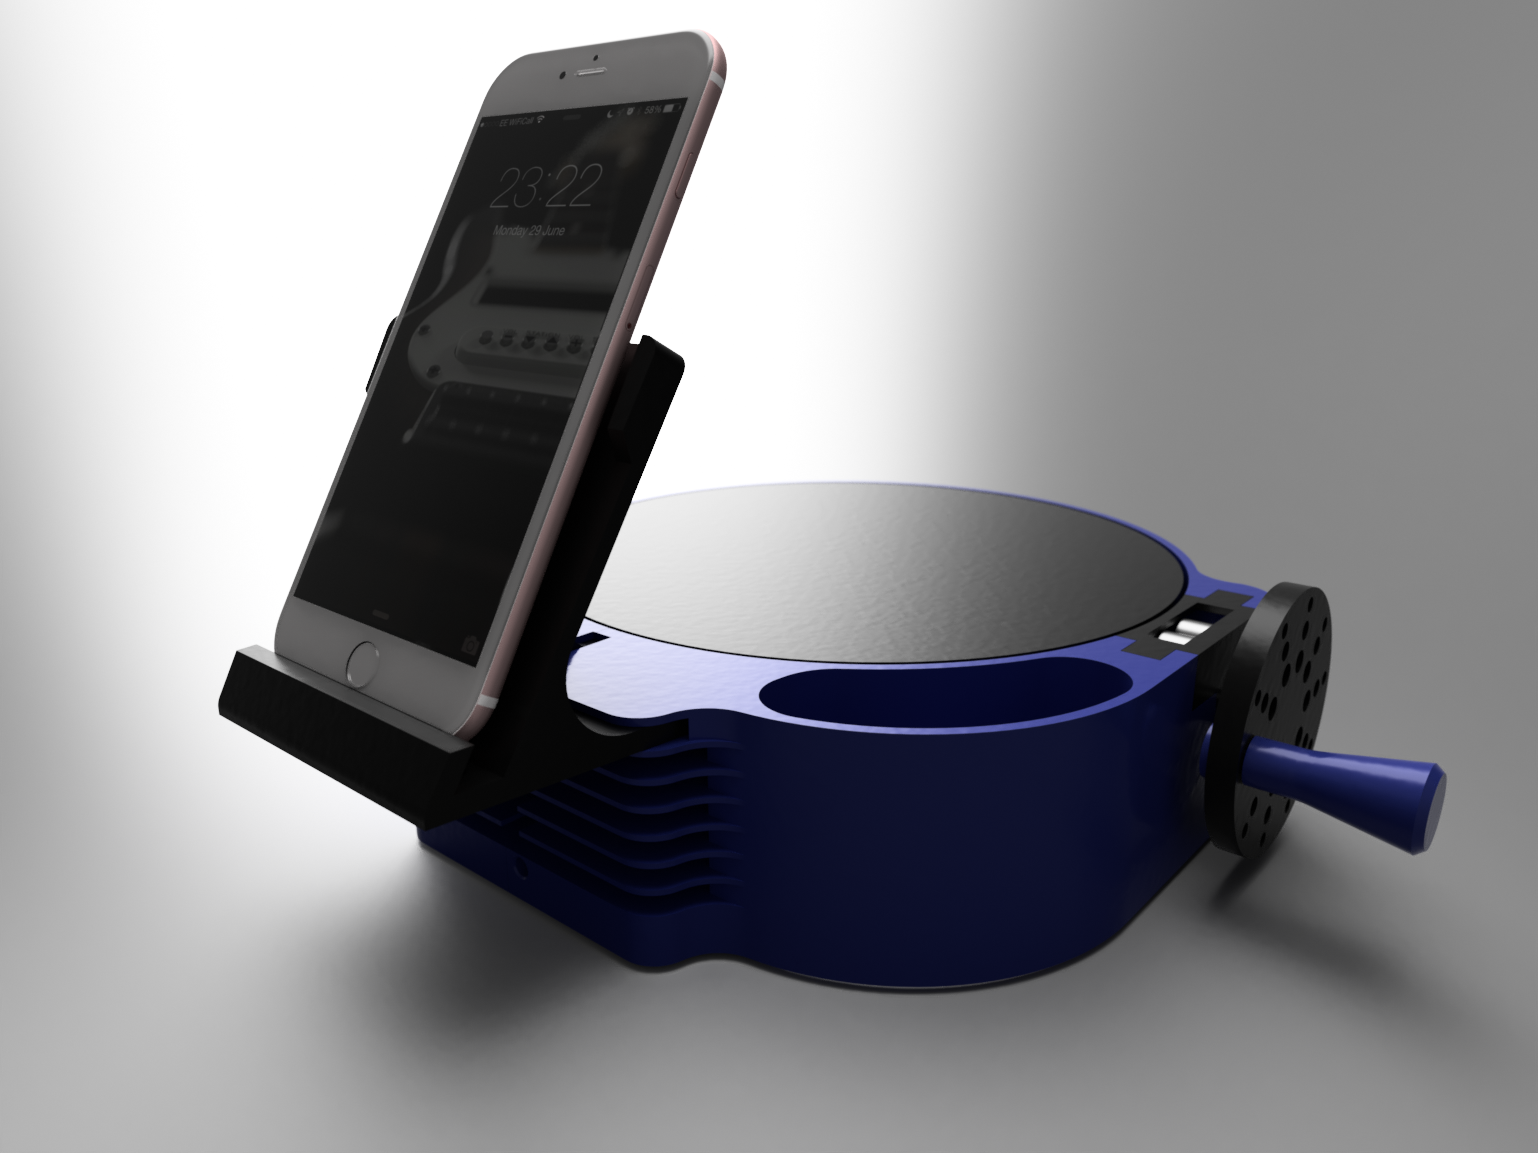
\includegraphics[width=\linewidth]{images/3DTurntable.png}\captionof{figure}{The 3D Scanner Turntable}}

It relies on the use of a smartphone camera and promises that only the filament costs (\SI[round-precision=2,round-mode=places,round-integer-to-decimal]{30}[\$]) will be incurred for the construction of the 3D scanner. In addition to the smartphone, matching headphones with buttons that allow the camera to be released are required.%

In order to achieve the goal of a 3D scanner that is as inexpensive as possible, the project does not use additional electronics that automate scanning. Instead, it is necessary for the user to turn a crank that rotates the object to be scanned and ensures that the smartphone takes 55 photos every full turn.%

Unlike the Open3DScanner or the OpenScan, the object is only rotated on one axis during the scan, so it may be necessary to perform several scans and reposition the object each time. It is therefore necessary for the user to interact more strongly with the 3D scanner during use, but this is the only way to keep costs so low compared to other projects.%

As with the OpenScan project, the captured images must then be processed with appropriate software in order to obtain a 3D model.%

\section{Ciclop}%
The Ciclop 3D Scanner is an ambitious project of Jesús Arroyo, published by bq and based on laser triangulation. In addition to the 3D scanner itself, the project also provides its own software (Windows, Linux, and Mac OS X) for performing the 3D scans.%

\hrefIdx{http://diwo.bq.com/en/einfuhrung-ciclop-und-horus/}{Ciclop}%
\marginElement{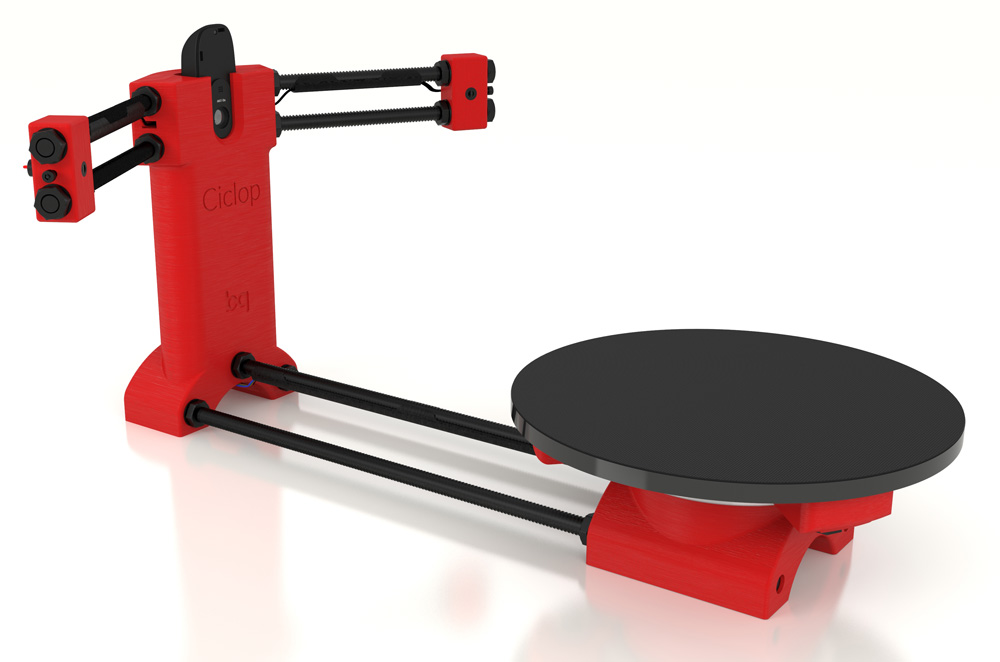
\includegraphics[width=\linewidth]{images/Ciclop.jpg}\captionof{figure}{The Ciclop 3D Scanner}}%

Even though this project has no influence on the development of the Open3DScanner, it shall be introduced briefly here, as it is a wonderful open source hardware project for the creation of a 3D scanner, which provides detailed source information and documentation.%

The result of a scan is a point cloud, which has to be converted into a 3D model with other software (e.g. \hrefIdx{https://www.blender.org/}{Blender}) before the model can be used further, e.g. for 3D printing.%

The whole project is published under the CC-BY-SA 3.0 license as well as the GPL v2.%

Unlike the previous projects, the Ciclop is not based on external hardware (like the camera of a smartphone), but is a complete project in itself, requiring only a PC for operation.%

The core of the project is formed by a \hrefIdx{https://www.logitech.com/en-us/product/hd-webcam-c270}{Logitech C270 HD webcam} for creating the photos and two class 1 lasers, which are used to sample the object. The object to be scanned is positioned on a plate which is automatically rotated.%